\documentclass[cs4size,a4paper]{ctexart}
%==================== 数学符号公式 ============
\usepackage{amsmath}                 % AMS LaTeX宏包
\usepackage[style=1]{mdframed}
\usepackage{amsthm}
\usepackage{amsfonts}
\usepackage{mathrsfs}                % 英文花体字 体
\usepackage{bm}                      % 数学公式中的黑斜体
\usepackage{bbding,manfnt}           % 一些图标,如 \dbend
\usepackage{lettrine}                % 首字下沉,命令\lettrine
\def\attention{\lettrine[lines=2,lraise=0,nindent=0em]{\large\textdbend\hspace{1mm}}{}}
\usepackage{longtable}
\usepackage[toc,page]{appendix}
\usepackage{geometry}                % 页边距调整
\usepackage{float}
\usepackage{amssymb}

\usepackage{amsmath}
\makeatletter
\newcommand{\rmnum}[1]{\romannumeral #1}
\newcommand{\Rmnum}[1]{\expandafter\@slowromancap\romannumeral #1@}
\makeatother
\geometry{top=3.0cm,bottom=2.7cm,left=2.5cm,right=2.5cm}
%====================公式按章编号==========================
\numberwithin{equation}{section}
\numberwithin{table}{section}
\numberwithin{figure}{section}
%================= 基本格式预置 ===========================
\usepackage{fancyhdr}
\pagestyle{fancy}
\fancyhf{}
\fancyhead[C]{\zihao{5}  \kaishu BOOTING A PC AND MEMORY MANAGEMENT }
\fancyfoot[C]{~\zihao{5} \thepage~}
\renewcommand{\headrulewidth}{0.65pt}
\CTEXsetup[format={\centering\bfseries\zihao{-2}},name={Chapter,}]{section}
\CTEXsetup[nameformat={\bfseries\zihao{3}}]{subsection}
\CTEXsetup[nameformat={\bfseries\zihao{4}}]{subsubsection}
%================== 图形支持宏包 =========================
\usepackage{subfigure}
\usepackage{graphicx}                % 嵌入png图像
\usepackage{color,xcolor}            % 支持彩色文本、底色、文本框等
\usepackage{hyperref}                % 交叉引用
\usepackage{caption}
\captionsetup{figurewithin=section}
%==================== 源码和流程图 =====================
\usepackage{listings}                % 粘贴源代码
\usepackage{xcolor}
\usepackage{color}
\definecolor{dkgreen}{rgb}{0,0.6,0}
\definecolor{gray}{rgb}{0.5,0.5,0.5}
\definecolor{mauve}{rgb}{0.58,0,0.82}
 \usepackage{xcolor}
 \lstset{
  %行号
    numbers=left,
    %背景框
    framexleftmargin=8mm,
    frame=none,
     %背景色
    %backgroundcolor=\color[rgb]{1,1,0.76},
     backgroundcolor=\color[RGB]{245,245,244},
     %样式
   keywordstyle=\bf\color{blue},
   identifierstyle=\bf,
    numberstyle=\color[RGB]{0,192,192},
    commentstyle=\it\color[RGB]{0,96,96},
   stringstyle=\rmfamily\slshape\color[RGB]{128,0,0},
   %显示空格
    showstringspaces=false
 }


%--------------------
\hypersetup{hidelinks}
\usepackage{booktabs}
\usepackage{shorttoc}
\usepackage{tabu,tikz}
\usepackage{float}

\usepackage{multirow}



\tabcolsep=1ex
\tabulinesep=\tabcolsep
\newlength\tikzboxwidth
\newlength\tikzboxheight
\newcommand\tikzbox[1]{%
        \settowidth\tikzboxwidth{#1}%
        \settoheight\tikzboxheight{#1}%
        \begin{tikzpicture}
        \path[use as bounding box]
                (-0.5\tikzboxwidth,-0.5\tikzboxheight)rectangle
                (0.5\tikzboxwidth,0.5\tikzboxheight);
        \node[inner sep=\tabcolsep+0.5\arrayrulewidth,line width=0.5mm,draw=black]
                at(0,0){#1};
        \end{tikzpicture}%
        }

\makeatletter
\def\hlinew#1{%
  \noalign{\ifnum0=`}\fi\hrule \@height #1 \futurelet
   \reserved@a\@xhline}

\newcommand{\tabincell}[2]{\begin{tabular}{@{}#1@{}}#2\end{tabular}}%

\usepackage{subfigure}

\usepackage{CJK}
\usepackage{ifthen}


\usepackage{graphicx}
\newcommand{\HRule}{\rule{\linewidth}{0.5mm}}

\newtheorem{Theorem}{定理}
\newtheorem{Lemma}{引理}
%%使得公式随章节自动编号
\makeatletter
\@addtoreset{equation}{section}
\makeatother
\renewcommand{\theequation}{\arabic{section}.\arabic{equation}}

%-------------------------
	
\usepackage{pythonhighlight}
\usepackage{tikz}
\usepackage{tikz-3dplot}
\usetikzlibrary{shapes,arrows,positioning}
%===================   正文开始    ===================
\begin{document}
\bibliographystyle{gbt7714-2005}     %论文引用格式
%===================  定理类环境定义 ===================
\newtheorem{example}{例}              % 整体编号
\newtheorem{algorithm}{算法}
\newtheorem{theorem}{定理}            % 按 section 编号
\newtheorem{definition}{定义}
\newtheorem{axiom}{公理}
\newtheorem{property}{性质}
\newtheorem{proposition}{命题}
\newtheorem{lemma}{引理}
\newtheorem{corollary}{推论}
\newtheorem{remark}{注解}
\newtheorem{condition}{条件}
\newtheorem{conclusion}{结论}
\newtheorem{assumption}{假设}
%==================重定义 ===================
\renewcommand{\contentsname}{CONTENTS}
\renewcommand{\abstractname}{摘要}
\renewcommand{\refname}{参考文献}
\renewcommand{\indexname}{索引}
\renewcommand{\figurename}{图}
\renewcommand{\tablename}{表}
\renewcommand{\appendixname}{附录}
\renewcommand{\proofname}{证明}
\renewcommand{\algorithm}{算法}
%============== 封皮和前言 =================
\begin{titlepage}

\begin{center}


% Upper part of the page

\includegraphics[width=0.8\textwidth]{figure/logoNankai}\\[1cm]

\textsc{\LARGE OPERATING SYSTEM }\\[1.5cm]

\textsc{\LARGE EXPERIMENTAL REPORT \Rmnum{1}}\\[0.5cm]


% Title
\HRule \\[0.8cm]
{\huge \bfseries BOOTING A PC AND MEMORY MANAGEMENT}\\[0.4cm]

\HRule \\[3.0cm]

% Author and major
\begin{minipage}{0.4\textwidth}
\begin{center}
Yinhao Li 1611303

Jiajun Li 1613368

Qiaoqiao Pan 1613415

Xinghe Li 1611071

Hongbo Xu 1611336
\end{center}
\end{minipage}

\vfill

% Bottom of the page


\end{center}

\end{titlepage}




\pagestyle{plain}
\pagenumbering{Roman}
%============== 摘要 ======================
\section*{\zihao{2} \centering \textbf{Abstract} }
   %用了Times New Roman字体来美化观感
Through the study of Experiment 1, we learned how the operating system works when the computer starts and how the computer manages the memory.

In Chapter 1, we will discuss Computer Boot, Boot Loader and The Kernel in detail. We will start research on the X86 assembly instructions, BIOS execution, PC physical address space, how the Boot Loader loads the kernel, the connection address and load address, the use of virtual memory, the formatted output of the console, and the stack.

In Chapter 2, we will discuss physical page management, virtual memory, and kernel address space. Describe in detail the relationship between virtual addresses and linear and physical addresses, reference counts, page table management, permissions and fault isolation, initialization of linear portions of the kernel, and so on.
\par
\vspace{3ex}
\textbf{Key Words:} Computer Boot\quad Boot Loader\quad The Kernel\quad physical page management\quad virtual memory\quad kernel address space
\addcontentsline{toc}{section}{Abstract}





\pagestyle{empty}
\tableofcontents
\thispagestyle{empty}


%============== 论文正文   =================
\pagestyle{fancy}
\pagenumbering{arabic}

\section{Booting a PC}

\subsection{Computer Boot }


\subsubsection{Simulating The X86}
In this experiment, we chose QEMU to simulate a real computer. The use of QEMU is as follows.
\begin{figure}[htbp]
\centering
\begin{minipage}[t]{0.48\textwidth}
\centering
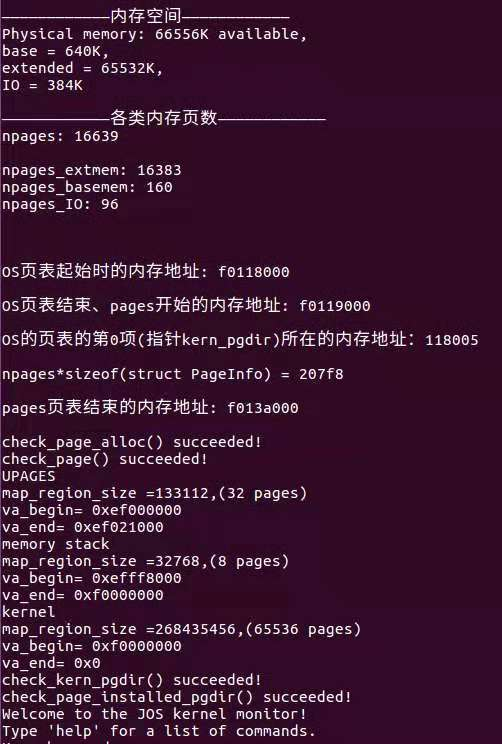
\includegraphics[width=6cm]{figure/make_qemu}
\caption{make qemu}
\end{minipage}
\begin{minipage}[t]{0.48\textwidth}
\centering
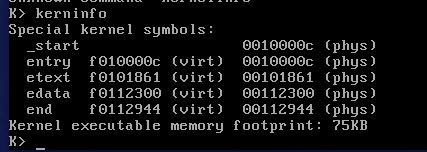
\includegraphics[width=6cm]{figure/kerninfo}
\caption{kerninfo}
\end{minipage}
\end{figure}

Through the above two instructions, we can see that the kernel information has been output in the console. It can be seen that QEMU can function as a simulation computer and the system can run normally.
\subsubsection{The PC's Physical Address Space}
The approximate physical distribution of the physical memory of the pc is as follows
\begin{figure}[H]
  \centering
  % Requires \usepackage{graphicx}
  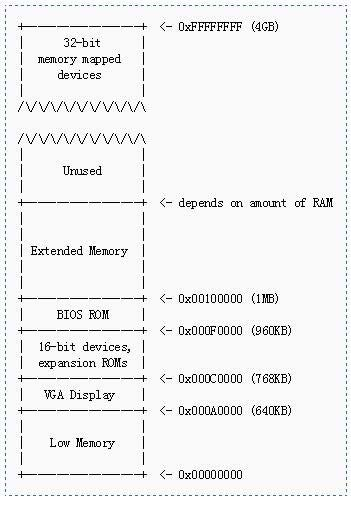
\includegraphics[width=0.8\linewidth]{figure/physical_address}\\
  \caption{i文件部分代码}\label{2}
\end{figure}
The 384KB of physical address range 0x000A0000~0x000FFFFF is reserved for hardware devices such as VGA display buffers. The most important part of this part is as the basic input and output system (BIOS, Basic)Input/Output System) The 64KB area of ​​0x000F0000~0x000FFFFF. The BIOS handles the basic initialization tasks of the system, such as activating the display, checking memory, and so on. After completing these initialization tasks, the BIOS loads the operating system from a floppy disk, hard drive, optical drive, or network and transfers control to the operating system.

On the modern PC, the 0x000A0000~0x00100000 segment is left as a "hole", which divides the memory into two segments. The lower 640K is called "low-segment memory", and the remaining high-address portion is expanded memory. At the same time, in the highest part of the physical address space, above all physical RAM, some are also reserved by the BIOS for 32-bit PCI devices.
\subsubsection{BIOS}
\begin{figure}[H]
  \centering
  % Requires \usepackage{graphicx}
  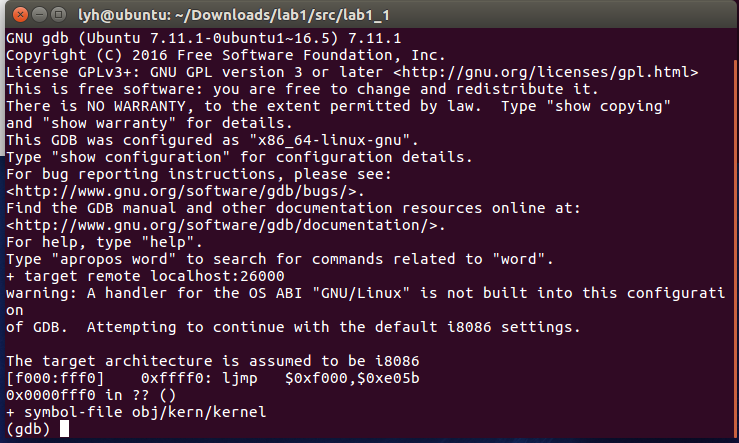
\includegraphics[width=0.8\linewidth]{figure/gdb}\\
  \caption{gdb}\label{2}
\end{figure}

In the running content of gdb, we can see the first instruction that gdb runs (as shown below). In this instruction, we can see that pc starts from CS = 0xf000 and IP = 0xfff0. The execution of the first sentence is a JMP operation that jumps to CS = 0xf000 and IP = 0xe05b. Since the modern CPU is divided into real mode and protection mode, it runs in real mode at startup and runs in protected mode after startup. The BIOS is the software that runs when the PC first starts up, so it must work in real mode. So the real address of the jump is 0xf000<<4+0xe05b = 0xfe05b.



\begin{figure}[H]
  \centering
  % Requires \usepackage{graphicx}
  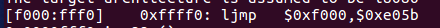
\includegraphics[width=0.8\linewidth]{figure/first_commond}\\
  \caption{The first instruction of the BIOS}\label{2}
\end{figure}


\subsection{Boot Loader}
For PCs, floppy disks and hard disks can be divided into 512-byte areas called sectors. A sector is the smallest granularity of a disk operation. Each read or write operation must be one or more sectors. If a disk can be used to boot the operating system, the first sector of the disk is called the boot sector. The boot loader program described in this section is located in this boot sector. When the BIOS finds a floppy disk or hard disk that can be booted, it loads the 512-byte boot sector into the memory address 0x7c00~0x7dff.
The boot loader must perform two main functions.

 1. First, the boot loader will convert the processor from real mode to 32-bit protected mode, because only in this mode the software can access more than 1MB of content.

 2. The boot loader can then access the IDE disk device registers directly from the disk by using x86 specific IO instructions.

For the boot loader, there is a file that is important, obj/boot/boot.asm. This file is a disassembled version of our real-run boot loader program. So we can compare it with its source code, boot.S and main.c.

\subsubsection{Question \Rmnum{1}}
Set a breakpoint at address 0x7c00, which is where the boot sector will be loaded. Continue execution until that breakpoint. Trace through the code in boot/boot.S, using the source code and the disassembly file obj/boot/boot.asm to keep track of where you are. Also use the x/i command in GDB to disassemble sequences of instructions in the boot loader, and compare the original boot loader source code with both the disassembly in obj/boot/boot.asm and GDB.

Trace into bootmain() in boot/main.c, and then into readsect(). Identify the exact assembly instructions that correspond to each of the statements in readsect(). Trace through the rest of readsect() and back out into bootmain(), and identify the begin and end of the for loop that reads the remaining sectors of the kernel from the disk. Find out what code will run when the loop is finished, set a breakpoint there, and continue to that breakpoint. Then step through the remainder of the boot loader.
\begin{flushleft}
1) At what point does the processor start executing 32-bit code? What exactly causes the switch from 16- to 32-bit mode?\\
2) What is the last instruction of the boot loader executed, and what is the first instruction of the kernel it just loaded?\\
3) Where is the first instruction of the kernel?\\
4) How does the boot loader decide how many sectors it must read in order to fetch the entire kernel from disk? Where does it find this
information?\\
\end{flushleft}

The BIOS will copy the boot sector to the address 0x7c00, so the starting address of boot.S is 0x7c00.So we enter b *0x7c00 in the gdb window, then enter c, which means continue to run to the breakpoint, where we enter x/30i 0x7c00.This gdb instruction disassembles the instructions stored in 0x7c00 and the next 30 bytes of memory.
\begin{figure}[H]
  \centering
  % Requires \usepackage{graphicx}
  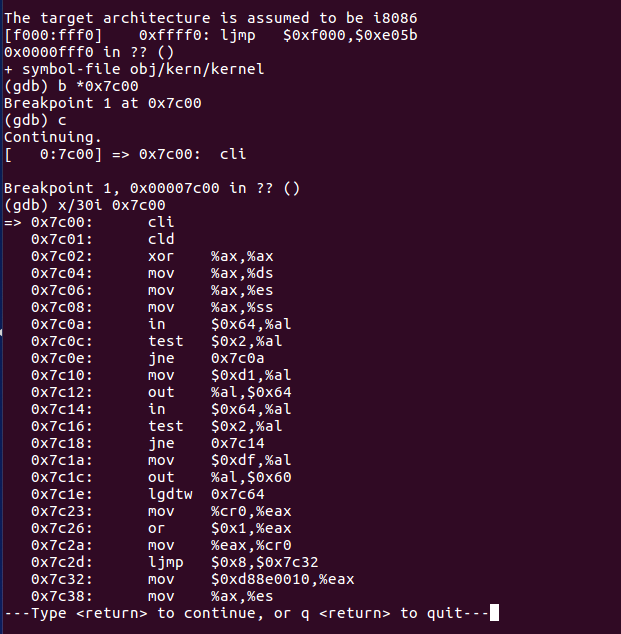
\includegraphics[width=0.8\linewidth]{figure/set_breakpoint}\\
  \caption{Disassembly}\label{2}
\end{figure}

We take it directly with boot.S and at obj/boot/boot.asm

\begin{figure}[H]
\centering
\begin{minipage}[t]{0.7\textwidth}
\centering
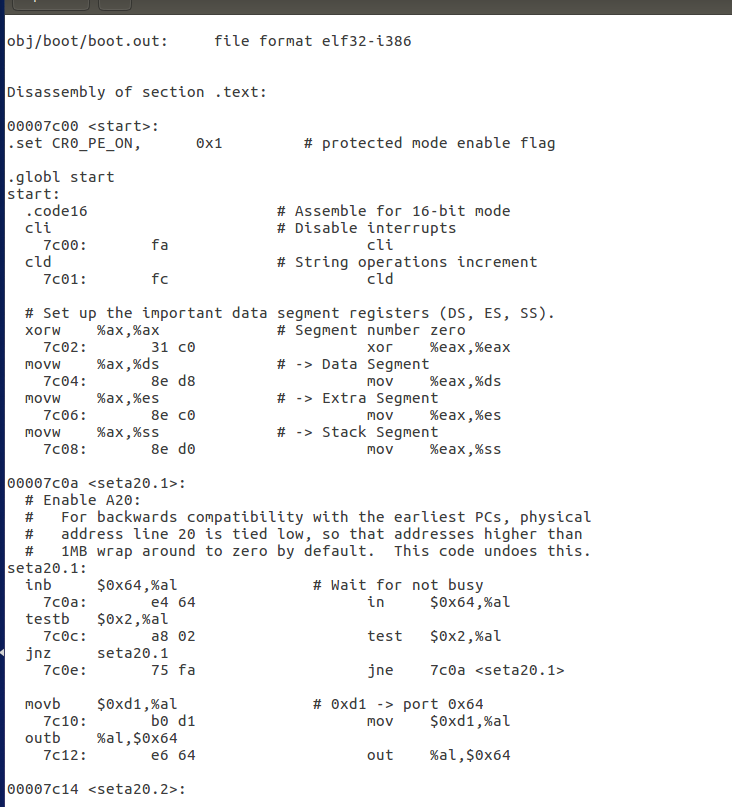
\includegraphics[width=10cm]{figure/boot_asm}
\caption{boot.asm}
\end{minipage}
\begin{minipage}[t]{0.7\textwidth}
\centering
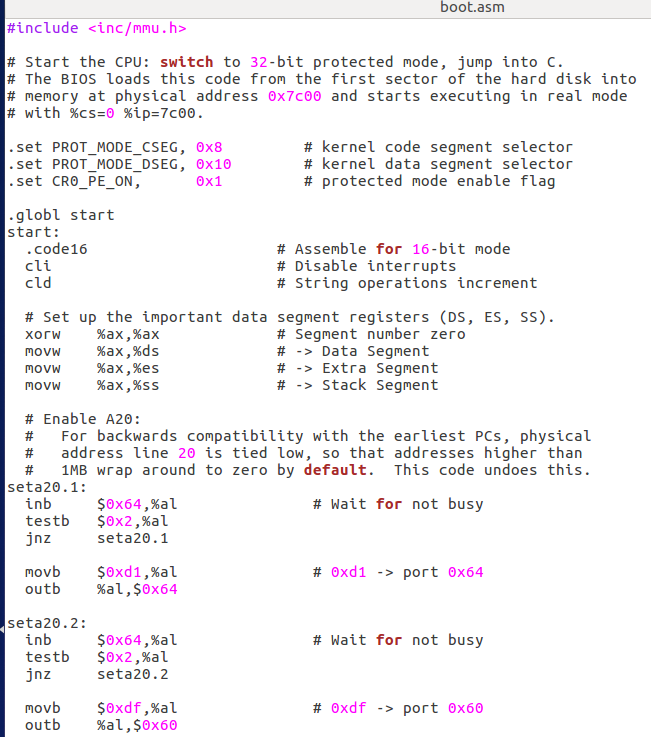
\includegraphics[width=10cm]{figure/boot_s}
\caption{boot.s}
\end{minipage}
\end{figure}

By comparing we can find that the three are not different in the instruction, but in the source code, we specify a lot of identifiers such as set20.1. Initially, these identifiers are converted to real physical addresses after being assembled into machine code. For example, set20.1 is converted to 0x7c0a, then this correspondence is listed in OBJ's /boot/boot.asm, but in the real case, in the first case, you can't see set20. 1 identifier, completely real physical address.


Then according to the title indication, we first traced to the bootmain function, we found that bootmain is at address 0x7c45, so we set the breakpoint there, and run here, then set the breakpoint at the readsect (0x7c7c) and jump here After using the si command to step through, found that into the waitdisk function (ox7c6a)
\begin{figure}[H]
  \centering
  % Requires \usepackage{graphicx}
  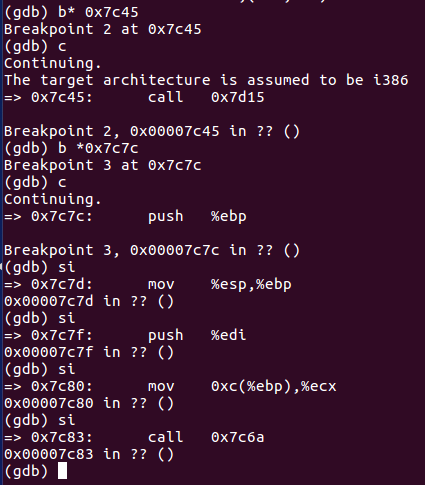
\includegraphics[width=0.8\linewidth]{figure/to_wait_disk}\\
  \caption{call bootmain}\label{2}
\end{figure}
In boot.asm we can find the corresponding content of 0x7d6b. Jumping to here means ((void (*)(void)) (ELFHDR->e\_entry))() the function is executed, where the meaning of the e\_entry field of the ELF header is the first instruction of the executable. Virtual address. So the meaning of this sentence is to transfer control to the operating system kernel.
Then we find the end of the for statement in the file and jump to this location (0x7d6b).
\begin{figure}[H]
  \centering
  % Requires \usepackage{graphicx}
  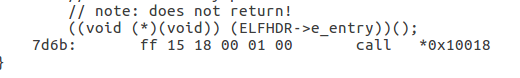
\includegraphics[width=0.8\linewidth]{figure/end_for}\\
  \caption{end loop}\label{2}
\end{figure}
\begin{figure}[H]
  \centering
  % Requires \usepackage{graphicx}
  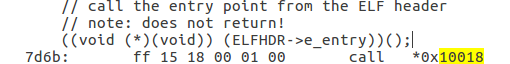
\includegraphics[width=0.8\linewidth]{figure/7d6b}\\
  \caption{the instruction after loop}\label{2}
\end{figure}
\vspace{9pt}
\begin{flushleft}
{\Large Answer:}\\
1)\\
\qquad As we discussed earlier, When the PC starts up, the CPU runs in real mode (real mode), and when it enters the operating system kernel, it will run in protected mode (protected mode). When entering protection mode, the CPU will switch from 16 bits to 32 bits.
\begin{figure}[H]
  \centering
  % Requires \usepackage{graphicx}
  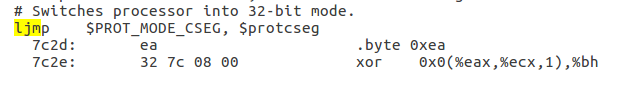
\includegraphics[width=0.8\linewidth]{figure/mode_change}\\
  \caption{mode change}\label{2}
\end{figure}
\qquad In the boot.S file, the computer first works in real mode, this time is the 16bit working mode. As can be seen from the above figure, when the "ljmp \$PROT\_MODE\_CSEG, \$protcseg" statement is run, the 32-bit working mode is officially entered. The root cause is that the CPU is working in protected mode at this time.\\
2)\\
\begin{figure}[H]
  \centering
  % Requires \usepackage{graphicx}
  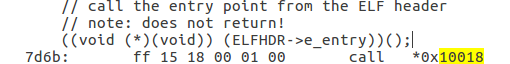
\includegraphics[width=0.8\linewidth]{figure/7d6b}\\
  \caption{the instruction after loop}\label{2}
\end{figure}
\qquad As shown in the figure above, the last statement executed by the boot loader is the last statement in the bootmain subroutine "((void (*)(void)) (ELFHDR->e\_entry))(); ", that is, jump to the operating system The starting instruction of the kernel program.
This first instruction is located in the /kern/entry.S file, the first sentence movw \$0x1234, 0x472\\
3)\\
\qquad The first instruction is in the /kern/entry.S file.\\
4)\\
\qquad First, how many segments are shared by the operating system, and how many sectors are in each segment are located in the Program Header Table in the operating system file. Each entry in this table corresponds to a segment of the operating system. And the content of each entry includes the size of the segment, the segment start address offset, and the like. So if we can find this table, we can determine how many sectors the kernel occupies by the information provided by the table entry.
Then the information about where this table is stored is stored in the ELF header information of the operating system kernel image file.\\
\end{flushleft}

\subsubsection{Loading kernel}
An executable ELF file consists of three main parts: a file header with loading information, followed by a program segment table, followed by several program segments. Each of these segments is a piece of continuous code or data. They are first loaded into memory when they are run. The job of the boot loader is to load them into memory.We can use the following instructions to examine the names, sizes, and addresses of all segments in the JOS kernel.

{\color{red} objdump -h obj/kern/kernel}

\begin{figure}[H]
  \centering
  % Requires \usepackage{graphicx}
  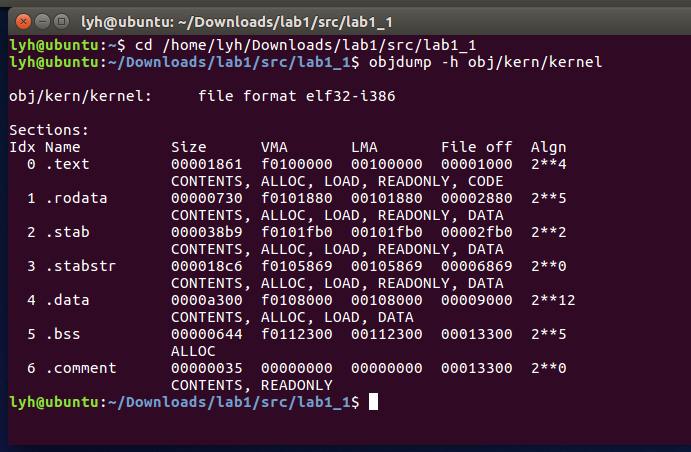
\includegraphics[width=0.8\linewidth]{figure/kernel_sections}
  \caption{All segment information in the kernel}\label{2}
\end{figure}

\subsubsection{Connection address and load address}
There are two more important fields in each segment, VMA (link address), LMA (load address). The load address represents the physical address of the segment after it is loaded into memory. The link address refers to the logical address to which this segment is expected to be stored.

Each ELF file has a Program Headers Table that indicates which parts of the ELF file are loaded into memory and the addresses that are loaded into memory. We get the information of the Program Headers Table of the kernel by entering the following instructions:

{\color{red} objdump -x obj/kern/kernel}
\begin{figure}[H]
  \centering
  % Requires \usepackage{graphicx}
  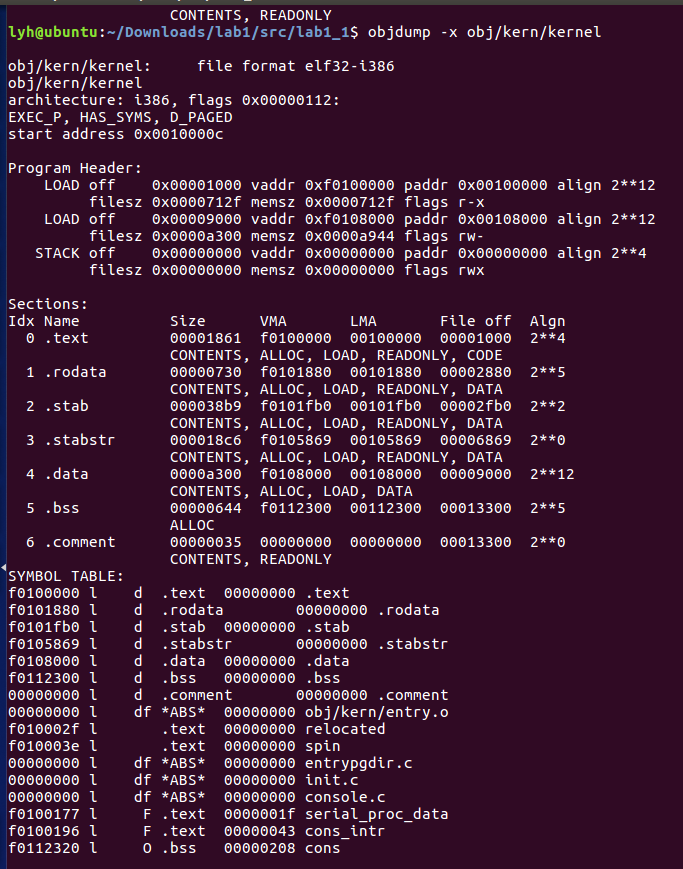
\includegraphics[width=0.8\linewidth]{figure/kernel_table}
  \caption{Kernel's Program Headers Table information}\label{2}
\end{figure}

\subsection{The Kernel}
\subsubsection{Question}
\begin{figure}[H]
  \centering
  % Requires \usepackage{graphicx}
  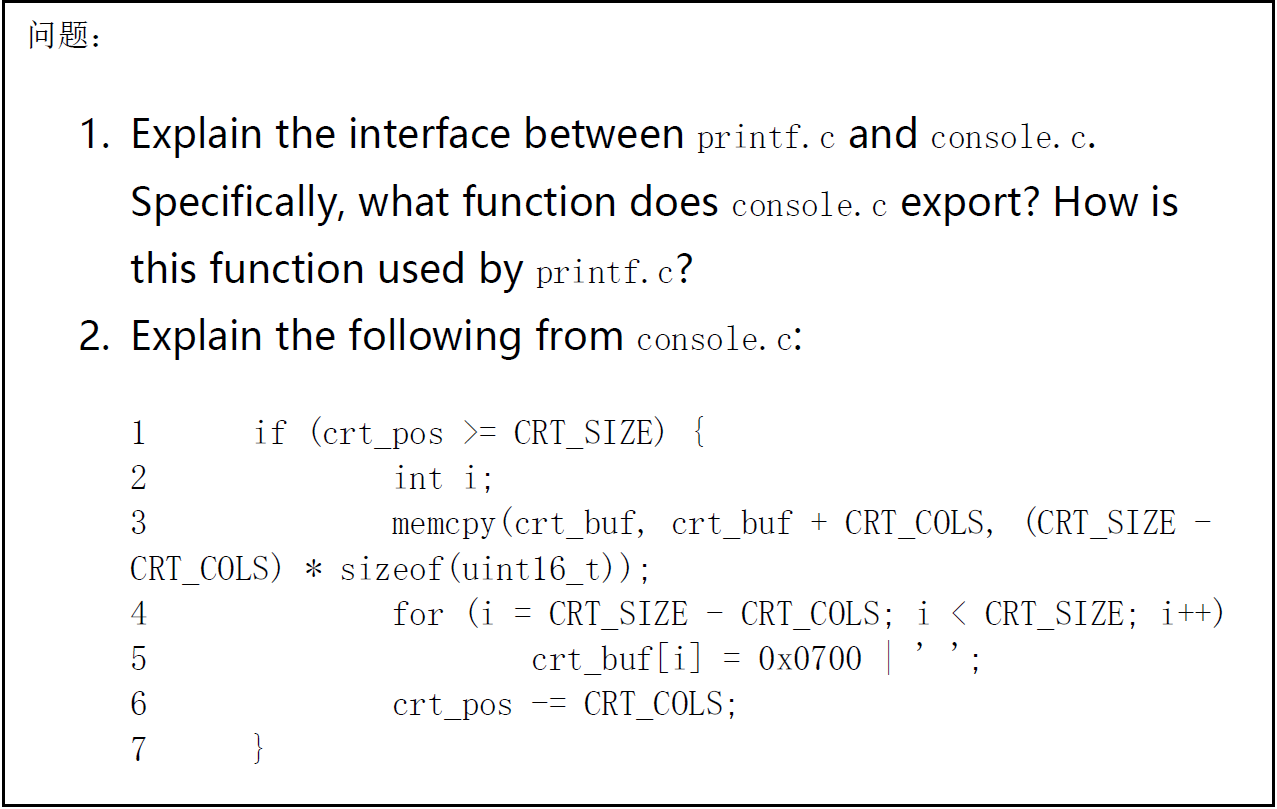
\includegraphics[width=0.8\linewidth]{figure/question}
\end{figure}
{\Large Answer:}\\
\begin{flushleft}
1)\\
\qquad Console.c defines how to display a character to the console, which is on top of our display, which includes many operations on the IO port.What is defined in printf.c is the top-level formatted output subroutine we will use in programming, such as printf, sprintf, and so on. The function exported by console.c which is used by printf.c is cputchar(),
That function prints a character in the parellel port and in the display.

\qquad Specific call relationship: cprintf -> vcprintf -> putch -> cputchar. Kernel's cprintf() function calls vprintfmt() (from lib/printfmt.c) to
Actually print in the console, vprintfmt() does the needed formatting and
Then call a function passed to it to actually print in the display.
\end{flushleft}
\begin{figure}[H]
  \centering
  % Requires \usepackage{graphicx}
  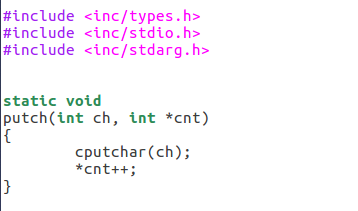
\includegraphics[width=0.8\linewidth]{figure/interface}
  \caption{Function call}\label{2}
\end{figure}
\begin{flushleft}
2)\\
\qquad Crt\_buf: This is a character array buffer that holds the characters to be displayed on the screen.\\

\qquad Crt\_pos: This indicates the position of the current last character displayed on the screen.\\
\qquad When crt\_pos >= CRT\_SIZE, where CRT\_SIZE = 80*25, since we know that the value range of crt\_pos is 0~(80*25-1), if this condition is true, it means that the content output on the screen has exceeded one page. . So at this point you have to scroll the page up one line, that is, put the original line 1~79 on the current 0~78 line, and then replace the line 79 with a line of spaces (of course not all spaces, 0 characters) To display the character int c) you entered. So the memcpy operation is to copy the contents of lines 1~79 in the crt\_buf character array to the position of lines 0~78. The next for loop is to turn the last line, line 79 into a space. Finally, you need to modify the value of crt\_pos.
\end{flushleft}

\subsubsection{Use virtual memory}
As we discussed earlier, the computer is divided into real mode and protected mode when it starts up.When running the boot loader, the link address (virtual address) and the load address (physical address) in the boot loader are the same. But when you enter the kernel, the two addresses are no longer the same.
In the virtual address space, we put the operating system at the high address 0xf0100000, but in the actual memory we store the operating system in a low physical address space, such as 0x00100000. Then when the user program wants to access an instruction of an operating system kernel, the first is to give a high virtual address, and then the virtual address is mapped to a real physical address by a certain mechanism in the computer, thus solving the above problem. . Then such an organization is usually implemented through segment management and paging management.
\subsubsection{Homework \Rmnum{1}}
{\Large We have omitted a small fragment of code - the code necessary to print octal numbers using patterns of the form "\%o". Find and fill in this code fragment.}

\begin{flushleft}
{\Large Answer}\\
\qquad To answer this question, we should first understand the three files $\backslash$ kern $\backslash$  printf.c, $\backslash$ kern $\backslash $ console.c, $\backslash$ lib $\backslash$ printfmt.c to understand the relationship between them.
\qquad First of all, we should pay attention to the console.c file, the most important of which is the cputchar subroutine. We can find that this program is the IO control program of the high-level console. In addition, the implementation of cputchar is actually done by calling cons\_putc. And the function of the cons\_putc program is to output a character to the console.
\end{flushleft}
\begin{figure}[H]
  \centering
  % Requires \usepackage{graphicx}
  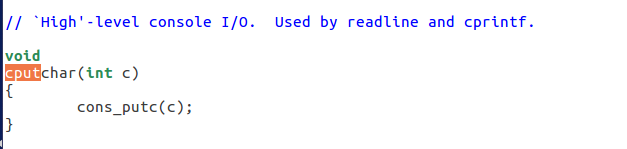
\includegraphics[width=0.8\linewidth]{figure/cputchar}
  \caption{cputchar}\label{2}
\end{figure}
\begin{figure}[H]
  \centering
  % Requires \usepackage{graphicx}
  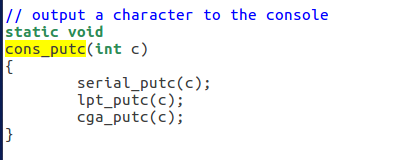
\includegraphics[width=0.8\linewidth]{figure/cons_putc}
  \caption{cons\_putc}\label{2}
\end{figure}
\qquad Then, let's focus on the printfmt.c file. By commenting, we can see that the subroutine defined in this file is the key to the information we can use to directly output information to the screen during programming using the printf function.
\begin{figure}[H]
  \centering
  % Requires \usepackage{graphicx}
  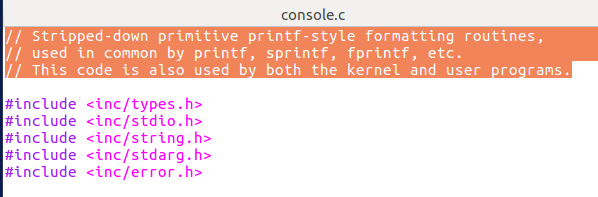
\includegraphics[width=0.8\linewidth]{figure/printfmt}
  \caption{printfmt}\label{2}
\end{figure}
Finally, let's take a look at the printf.c file.By commenting, we can see that the function of this file is to implement the simple implementation of cprintf console output for the kernel.
\begin{figure}[H]
  \centering
  % Requires \usepackage{graphicx}
  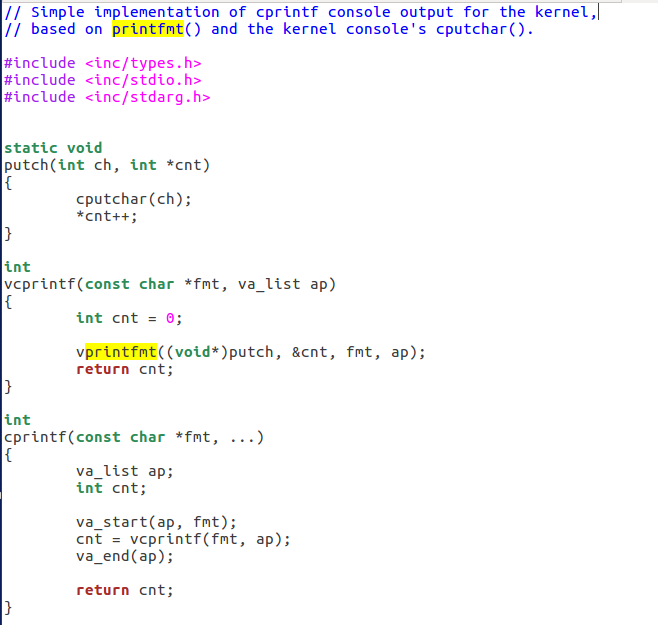
\includegraphics[width=0.8\linewidth]{figure/printf}
  \caption{printf}\label{2}
\end{figure}

In this question, we follow the case 'u' to write the code.
\begin{figure}[H]
  \centering
  % Requires \usepackage{graphicx}
  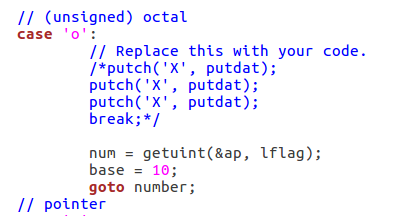
\includegraphics[width=0.8\linewidth]{figure/caseo}
  \caption{answer}\label{2}
\end{figure}

After that we modify the monitor.c file and then run qemu on the terminal to test our results.
\begin{figure}[H]
  \centering
  % Requires \usepackage{graphicx}
  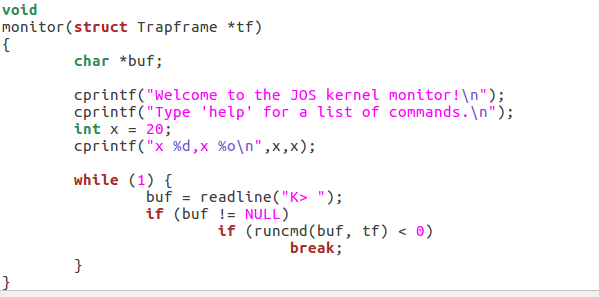
\includegraphics[width=0.8\linewidth]{figure/monitor}
  \caption{Change monitor}\label{2}
\end{figure}
\begin{figure}[H]
  \centering
  % Requires \usepackage{graphicx}
  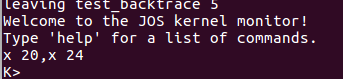
\includegraphics[width=0.8\linewidth]{figure/resultofmonitor}
  \caption{Result test}\label{2}
\end{figure}


As can be seen from the results, the 20 we defined is under \%d, and the \%o is correctly changed to octal 24

\subsubsection{Stack}
\begin{flushleft}
{\Large Exercise}

\qquad To become familiar with the C calling conventions on the x86,find the address of the test\_backtrace function in obj/kern/kernel.asm,set a breakpoint there,and examine what happens each time it gets called after the kernel starts.How many 32-bits words does each recursive nesting level of test\_backtrace push on the stack,and what are those words?\\


{\Large Answer}\\
\end{flushleft}

First, let's take a look at the source code of the test\_backtrace function in kernel.asm
\begin{figure}[H]
  \centering
  % Requires \usepackage{graphicx}
  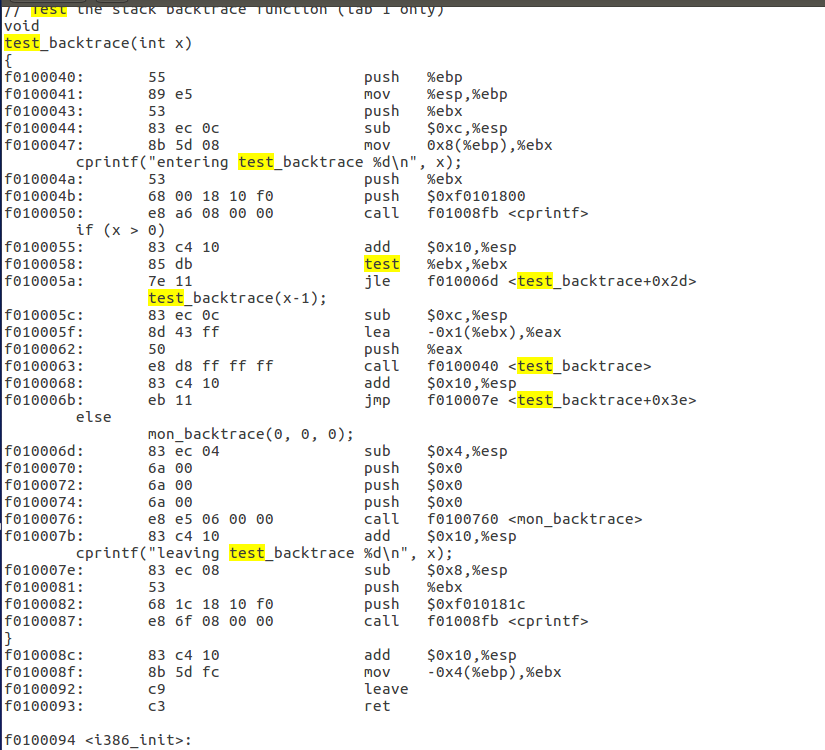
\includegraphics[width=0.8\linewidth]{figure/test_backtrace}
\end{figure}

From the code we can see the address of test\_backtrace, so we set a breakpoint here, then jump to here, as shown below:
\begin{figure}[H]
  \centering
  % Requires \usepackage{graphicx}
  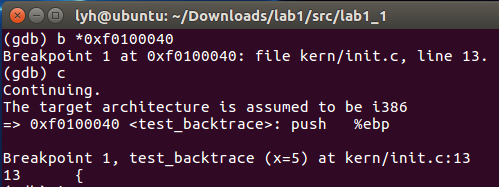
\includegraphics[width=0.8\linewidth]{figure/backtrace_set_breakpoint}
\end{figure}
Then we use the i r instruction to view the register contents and repeat the above operation
\begin{figure}[H]
  \centering
  % Requires \usepackage{graphicx}
  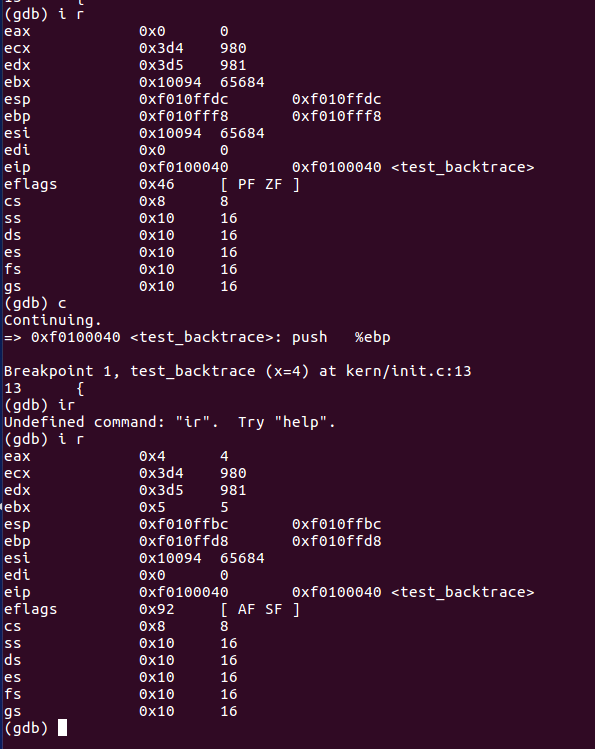
\includegraphics[width=0.8\linewidth]{figure/test_backtrace_c}
\end{figure}

By comparison, we can find that the value of ebp is reduced by 20 (hexadecimal), so we can judge every time it pushes 8 4-byte words.

According to the structure of the test\_backtrace function and the change of the stack when the function is called, each time the function is called, the ebp, the return address, the saved ebx value, and the parameters of the next call function must be pushed onto the stack. There are also 4 reserved words.

\subsubsection{Homework \Rmnum{2}}
\begin{flushleft}
{\Large Question}
\end{flushleft}

You can do mon\_backtrace() entirely in C.You'll also have to hook this new function into the kernel monitor's command list so that it can be invoked interactively by the user.The backtrace function should display a listing of function call frames in the following format:

Waring:

read\_ebp

display format

\begin{flushleft}
{\Large Answer}
\end{flushleft}



We first call the read\_ebp function to get the value of the current EBP register. We treat the entire call stack as an array, EBP[0] represents the ebp value of the previous function, and EBP [1] stores the function return address, EBP [2] What is stored later is the value of the input parameter.

\begin{table}[H]
\centering
\begin{tabular}{ |p{150pt}| }\toprule
\hline			
Ebp of the previous function  \\ \hline		
ebx \\ \hline 		
Parameter 1 \\ \hline 	
Parameter 2 \\ \hline
Parameter 3 \\ \hline
Parameter 4 \\ \hline
Parameter 5 \\ \hline
\end{tabular}
\caption{Stack structure diagram}
\end{table}

The modified mon\_backtrace function code is shown in the figure
\begin{figure}[H]
  \centering
  % Requires \usepackage{graphicx}
  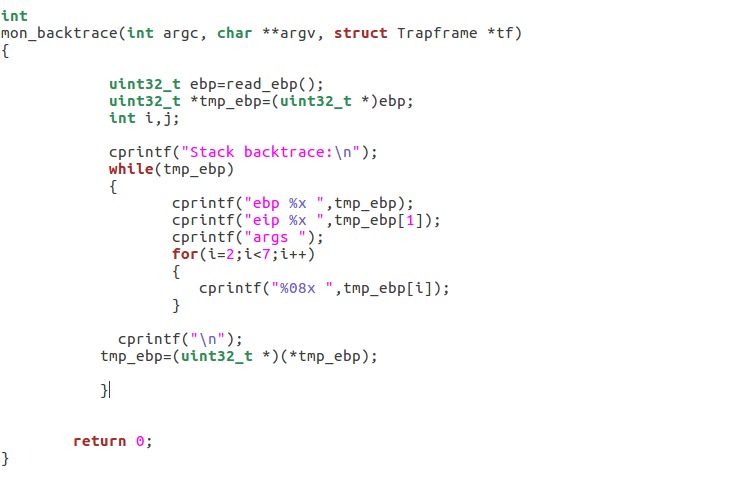
\includegraphics[width=0.8\linewidth]{figure/mon_backtrace_code}
\end{figure}

After analysis, we can know that when the function is called, the parameters are first pushed onto the stack, then the eip is pushed onto the stack, and finally the ebp is pushed onto the stack, and the new ebp points to the position of the old ebp. Therefore, the location pointed to by ebp stores the value of the previous function ebp, and the location of ebp+1 stores the value of eip. So we first print out tmp\_ebp as ebp, tmp\_ebp[1] as eip. Then we print out the values ​​of 5 parameters according to the requirements of the topic. Finally, we take the value in the memory space pointed to by ebp and repeat the above process until the first function is called.

The result of the operation is as follows
\begin{figure}[H]
  \centering
  % Requires \usepackage{graphicx}
  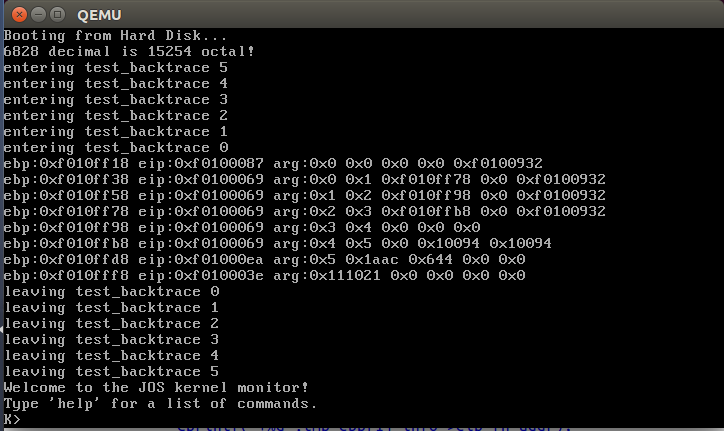
\includegraphics[width=0.8\linewidth]{figure/mon_backtrace_qemu}
\end{figure}

Add backtrace to the command list
\begin{figure}[H]
  \centering
  % Requires \usepackage{graphicx}
  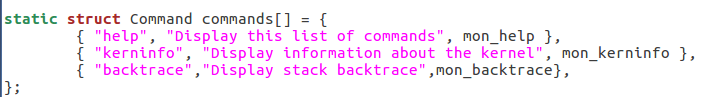
\includegraphics[width=0.8\linewidth]{figure/add_backtrace}
\end{figure}

The results are as follows:
\begin{figure}[H]
  \centering
  % Requires \usepackage{graphicx}
  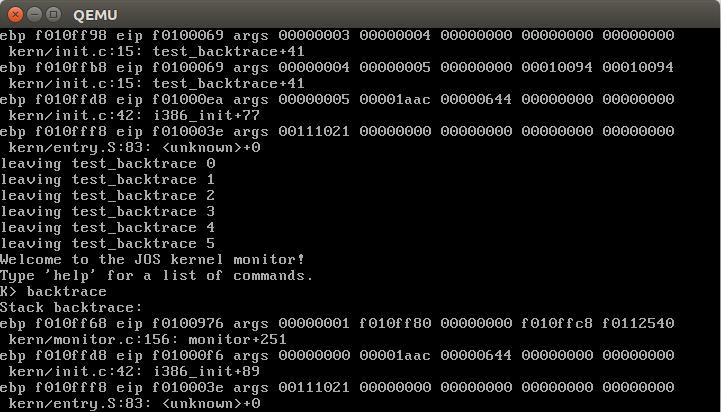
\includegraphics[width=0.8\linewidth]{figure/backtrace_result}
\end{figure}
\subsubsection{Challenge homework}
\begin{flushleft}
{\Large Question}
\end{flushleft}

Modify your stack backtrace function to display, for each eip, the function name, source file name, and line number corresponding to that eip.
In debuginfo\_eip, where do \_\_STAB\_* come from?

\begin{flushleft}
{\Large Answer}
\end{flushleft}


After reading the contents of stab.h and using the objdump -G kernel command, you can roughly know the fields of the stab table that store debugging information and their meanings, as follows

Uint32\_t n\_strx; index, can be added to stabstr to get the corresponding address of the string information.

Uint8\_t n\_type; The type of the line content, such as functions, function parameters, a line in the source file, etc.

Uint8\_t n\_other; usually empty.

Uint16\_t n\_desc; Stores the specific number of rows when type is n\_sline.

Uintptr\_t n\_value; The position of the corresponding content runtime in memory (or relative to the location where the function starts the instruction).

Collect the contents of the header file and the stab table, and analyze the meaning of each field as follows:
\begin{figure}[H]
  \centering
  % Requires \usepackage{graphicx}
  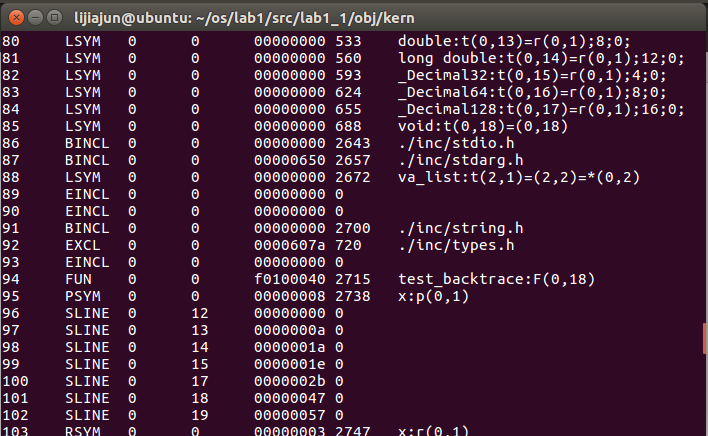
\includegraphics[width=0.8\linewidth]{figure/challenge_1}
\end{figure}

The function for finding symbol information is debuginfo\_eip(uintptr\_t addr, struct Eipdebuginfo *info)
Analyze kdbug.h, we found that the function of this function is to fill the corresponding fields of the Eipdebuginfo structure.
Analyze the debuginfo\_eip function,we find that its execution logic is roughly: the structure of the eip value to be searched and the information to save the result. In the stab table, a binary search is performed on the item whose n\_type is file, and it is found that the value of the eip is in the middle of the label of the two source files (the first item in the figure). Then, the labels of the two source files are used as the left and right intervals, and the items in which the type is fun are binary searched, and the value is found between the two function labels. Finally, the eip value is subtracted from the left interval function value, and a binary search is performed to find the corresponding eip line number.
The added code is as follows:
\begin{figure}[H]
  \centering
  % Requires \usepackage{graphicx}
  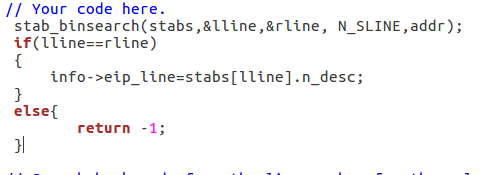
\includegraphics[width=0.8\linewidth]{figure/challenge_2}
\end{figure}


Modify the mon\_backtrace code to output the search result
\begin{figure}[H]
  \centering
  % Requires \usepackage{graphicx}
  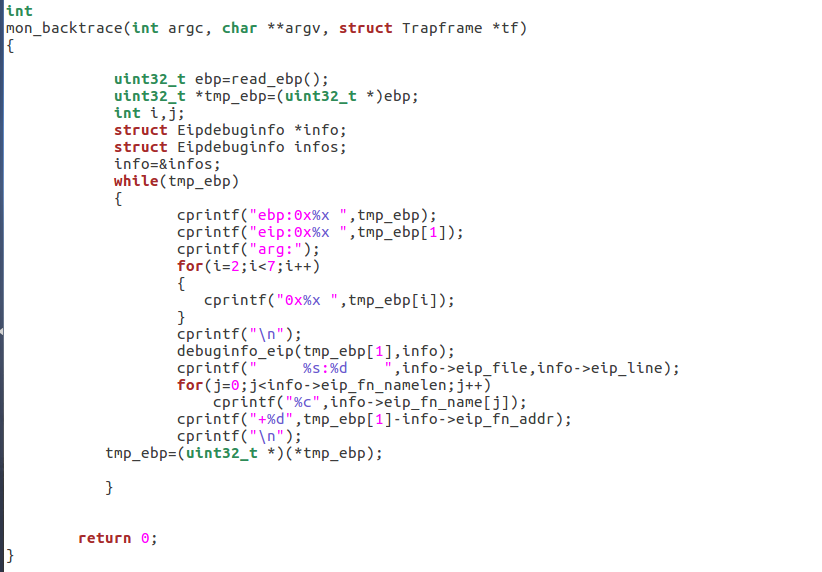
\includegraphics[width=0.8\linewidth]{figure/challenge_3}
\end{figure}

Eip\_fn\_namelen is used to exclude colon information after the function name

Tmp\_ebp[1](eip)-info->eip\_fn\_addr outputs the byte difference between the current instruction and the first instruction address of the function.

Source of \_\_STAB\_ * in debuginfo\_eip:

\begin{figure}[H]
  \centering
  % Requires \usepackage{graphicx}
  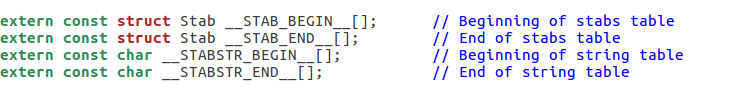
\includegraphics[width=0.8\linewidth]{figure/challenge_4}
\end{figure}


In kdebug.c, these variables are declared as extern, and their definitions are in kernel.ld as follows:

\begin{figure}[H]
  \centering
  % Requires \usepackage{graphicx}
  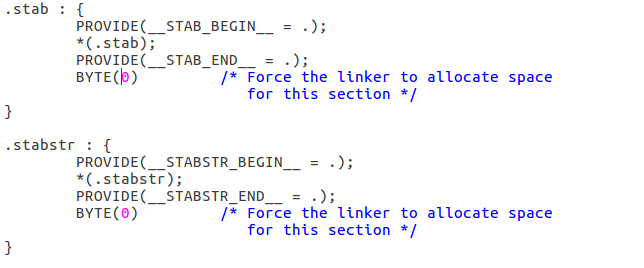
\includegraphics[width=0.8\linewidth]{figure/challenge_5}
\end{figure}

Taking the .stab section as an example, first define the \_\_STAB\_BEGIN\_\_ variable through PROVIDE, its address points to the beginning of the stab section, and then merge the stab sections of each file by the *(.stab) command (the section is compiled by the compiler when compiling each file). Generate, there are debugging information related to each file), and finally define the \_\_STAB\_END\_\_ variable, its position points to the end. The .stabstr section has the same definition as .stab.
\clearpage






























%\pagenumbering{arabic}

\section{Memory Management}
\subsection{Physical Page Management}
\subsubsection{Homework \Rmnum{3}}
\begin{flushleft}
{\Large Question}
\end{flushleft}

In the file kern/pmap.c, you need to implement the code for the following function (see below, given in order):

Boot\_alloc()

Mem\_init() (before calling check\_page\_free\_list(1))

Page\_init()

Page\_alloc()

Page\_free()

Check\_page\_free\_list() and check\_page\_alloc() will test your physical page allocator. You need to guide JOS

Then check the success report for check\_page\_alloc(). It would be helpful to add your own assert() to verify that your assumptions are correct.
\begin{flushleft}
{\Large Theoretical preparation}
\end{flushleft}


The operating system must keep track of which memory regions are free and which are occupied. The JOS kernel manages memory with the minimum granularity of pages (pages), which uses the MMU to map and protect the memory allocated for each block.

Here we have to write the allocation subfunction of the physical memory page. It uses a linked list of structure PageInfo to record which pages are free, and each node in the linked list corresponds to a physical page.

\begin{flushleft}
{\Large Analysis \& Answer}
\end{flushleft}

The operating system must keep track of which physical RAM is free and which is in use. This exercise mainly writes a physical page allocator. It uses a linked list of PageInfo structures to record which pages are free, and each structure corresponds to a physical page.

Because the implementation of the page table requires the allocation of physical memory to store the page table, we need to write the physical page allocator before the implementation of the virtual memory.
\begin{figure}[H]
\centering
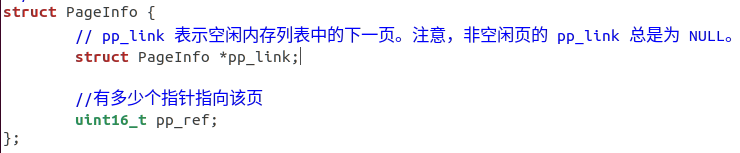
\includegraphics[width=0.8\linewidth]{figure/PageInfo}
\caption{Definition of PageInfo in memlayout.h}
\end{figure}


In the file kern/pmap.c, the function mem\_init() is called when the kernel first starts running, and some initialization settings are made for the memory management system of the entire operating system.

[Step 1] Enter mem\_init(). The first step is to call the sub-function i386\_detect\_memory() to check how much total memory space is available in the system and how much the three parts of the memory space are, and divide the page according to the set PGSIZE. The total number of pages and the number of pages in each of the three parts are calculated in the function.

JOS divides the entire physical memory space into three parts:

1 Basemen: Available from 0x00000 to 0xA0000

2 IO hole: From 0xA0000 to 0x100000, not available, mainly used to allocate to external devices.

3 Extmen: From 0x100000 to 0x, available, the most important memory area.

\begin{figure}[H]
\centering
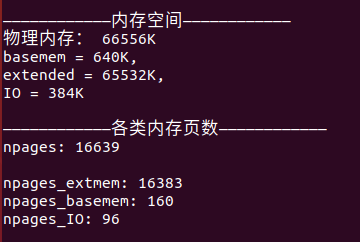
\includegraphics[width=0.8\linewidth]{figure/i386_detect_memory}
\caption{i386\_detect\_memory() run result}
\end{figure}

[Step 2] (1) Call the function boot\_alloc function to allocate a virtual memory of size PGSIZE followed by the operating system kernel bss for storing the operating system page table. When the operating system is working in virtual memory mode, this page directory table is required for address translation (virtual address→physical address).
The boot\_alloc function can be used to allocate virtual memory, and its parameter is the virtual memory byte size to be allocated. When 0 is input, the currently used virtual memory tail can be queried. The core idea of ​​this function is to maintain a static variable nextfree, which stores the virtual address corresponding to the next free memory space that can be used. The first time you enter the function you need to initialize nextfree. Note: The allocated memory size needs to be aligned with PGSIZE by the ROUNDUP function.

\begin{figure}[H]
\centering
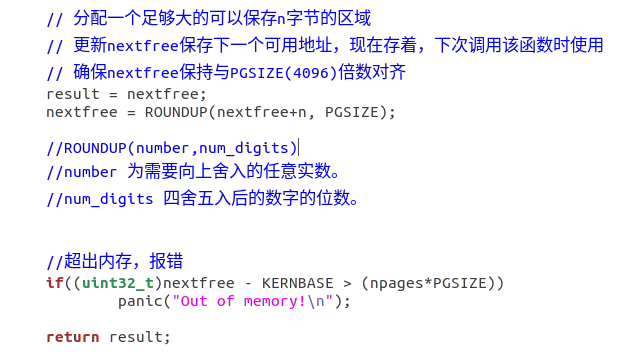
\includegraphics[width=0.8\linewidth]{figure/boot_alloc_changed}
\caption{The code supplemented by the boot\_alloc() function}
\end{figure}

(2) Initialize a pointer in physical memory kern\_pgdir points to the above operating system page table.

(3) Call the memset function to clear the virtual memory of the operating system page table area.

\begin{figure}[H]
\centering
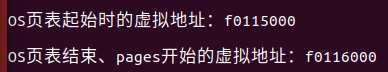
\includegraphics[width=0.8\linewidth]{figure/PGSIZE}
\caption{By information printing, the OS page table end address - OS page table start address = PGSIZE}
\end{figure}


[Step 3] Add the first page directory entry for the page directory table just created, occupying the 0th position of the page table. The content of the entry is the real address of the pointer kern\_pgdir. UVPT is defined as the starting address of a virtual address, 0xef400000. Starting from this virtual address, the page table kern\_pgdir of this operating system is stored, so we must map it to the physical address of the page table kern\_pgdir, PADDR(kern\_pgdir) It is calculating the real physical address corresponding to kern\_pgdir.
\begin{figure}[H]
\centering
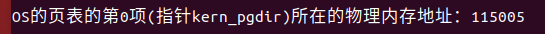
\includegraphics[width=0.8\linewidth]{figure/real_physical_address}
\caption{The actual physical address of the pointer is known by information printing.}
\end{figure}

[Step 4] Use the boot\_alloc function to allocate a virtual memory of size npages * sizeof(struct PageInfo), which is used to store an array of struct PageInfo. The pointers in memory point to the virtual memory. The OS uses this array to track the usage of all memory pages. Each PageInfo represents a page in memory. PageInfo has two attributes: 1. Whether the current page is occupied. 2. Pointer to the next page. Then call the memset function to clear the corresponding area memory.

\begin{figure}[H]
\centering
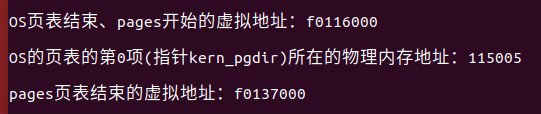
\includegraphics[width=0.8\linewidth]{figure/pages_alloc_virtualmem}
\caption{Allocate virtual memory for pages}
\end{figure}

Note: It is found through information printing that the memory address at the end of the pages page table minus the memory address at the beginning of the pages is not exactly equal to npages * sizeof(struct PageInfo), but slightly larger than when the virtual memory is allocated in the boot\_alloc function. It needs to be noted that it is aligned with the PGSIZE multiple, so the allocated virtual memory size is appropriately allocated upwards.

[Step 5] Call the function page\_init() to initialize the linked list of two struct pageinfo pages and page\_free\_list. The pages\_free\_list linked list stores all the free page information, and the pages store the information of the free\\non-free pages.

Jos divides the entire physical memory space into three parts, namely BASEMEM, IO HOLE, and EXTMEM.

According to the first item of the known basemem is already occupied, and other pages of basemem are not occupied. Since IO HOLE is mainly used to be allocated to external devices and is not available, it is equivalent to occupying all pages. EXTMEM is occupied in the first part of the page in step four, and part of it is idle.
\begin{figure}[H]
\centering
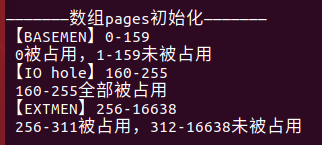
\includegraphics[width=0.8\linewidth]{figure/pages_init}
\caption{Pages initialization result}
\end{figure}

\begin{figure}[H]
\centering
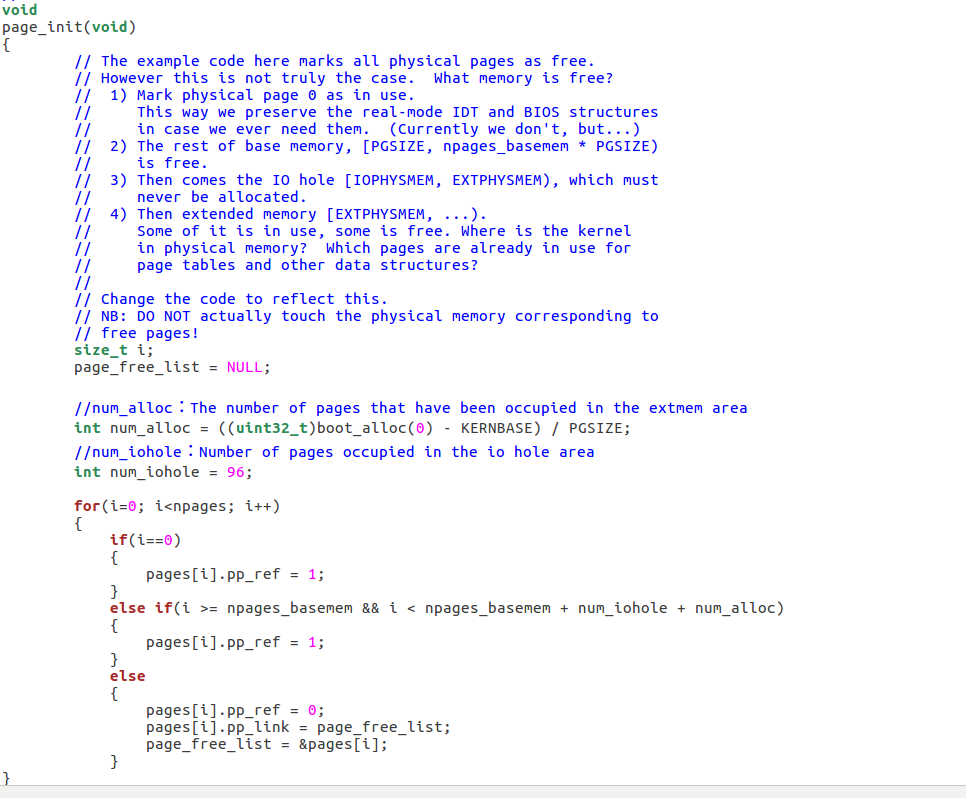
\includegraphics[width=0.8\linewidth]{figure/page_init_changed}
\caption{page\_init() supplemental code screenshot}
\end{figure}

[Step 6] Call check\_page\_free\_list() and check\_page\_alloc() to test the above physical page allocator.

Check\_page\_free\_list() checks whether the so-called free pages of the page\_free\_list linked list are really legal and free. When the input parameter is 1, this function needs to perform one additional operation before checking, and modify the free page list free\_page\_list. After page\_init, free\_page\_list has stored all the free page tables, but their order is according to the page table. The numbers are arranged from large to small. In the page directory table entry\_pgdir (not kern\_pgdir) used by the current operating system, the page table of the large number is not mapped, so we cannot operate this part of the page table. However, the small numbered page table, that is, from the page table 0 to the page table 1023, has been mapped, so this page table can be operated. Then check\_page\_free\_list(1) is to complete the PageInfo structure corresponding to this part of the page table to the front end of the free\_page\_list for the operating system to use now. The rest of the operation is to check the free\_page\_list.

The function of the check\_page\_alloc() function is to check if page\_alloc() and page\_free() functions correctly.

One of the job requirements is to implement the page\_alloc() function. By commenting we can know that the function of this function is to allocate a physical page. The return value of the function is the PageInfo structure corresponding to this physical page. So the general steps of this function should be:

1. Take a PageInfo structure of a free page from free\_page\_list

2. Modify the free\_page\_list related information, such as modifying the linked list header

3. Modify the PageInfo structure information of the taken free page to initialize the memory of the page.

\begin{figure}[H]
\centering
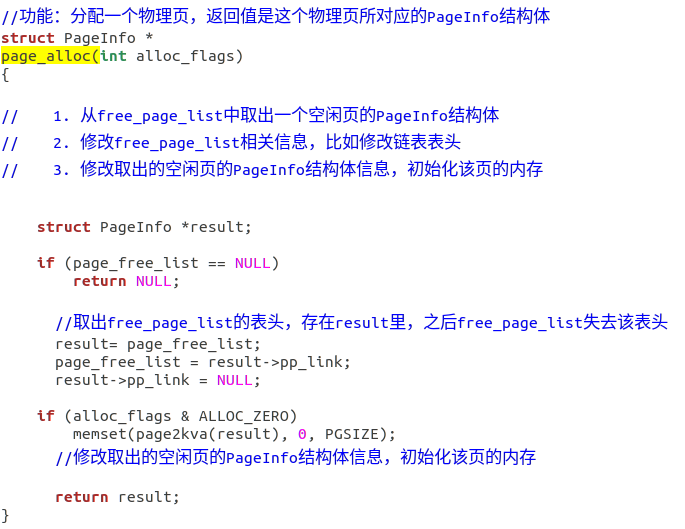
\includegraphics[width=0.8\linewidth]{figure/page_alloc_changed}
\caption{Page\_alloc() function complement code}
\end{figure}

Similarly, the job requires page\_free(). According to the comment, the function of this method is to return the PageInfo structure of a page to the page\_free\_list free page list, which means that the page is recycled. Mainly complete the following operations:

1. Modify the corresponding information of the PageInfo structure of the page being recycled.

2. Insert the structure back into the page\_free\_list free page list
\begin{figure}[H]
\centering
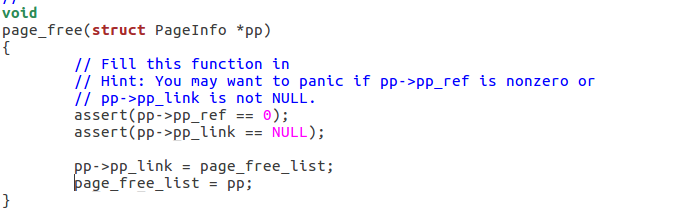
\includegraphics[width=0.8\linewidth]{figure/page_free_changed}
\caption{Page\_free function supplement code}
\end{figure}
\subsection{Virtual Memory}
\subsubsection{Exercise \Rmnum{4}}
\begin{flushleft}
{\Large Question}
\end{flushleft}

Read Chapters 5 and 6 of the Intel 80386 Reference Manual for reading about page conversion and page-based protection(5.2 and 6.4). We recommend that you briefly understand the chapter on segmentation mode, because although the use of JOS is based on
Page memory for virtual memory and protection, but segment conversion and segment-based protection cannot be disabled on x86, so you need
Have a basic understanding..

\begin{flushleft}
{\Large Answer}
\end{flushleft}

The logical address of the page consists of the page number and the in-page address

The physical address of the page is spliced ​​by the block number and the address within the page.

The purpose of the page table is to implement address mapping from page number to physical block number. The page table is retrieved by the page number of the logical address to obtain the physical block number of the page; and the in-page address d is directly sent into the block address field of the physical address register. In this way, the physical block number and the intra-block address are spliced ​​into an address that actually accesses the memory, thereby completing the conversion from the logical address to the physical address.

So the calculation formula for the physical address is:

Physical address = block size (ie page size L) ́ block number f + page address d

\subsubsection{Virtual address, linear address and physical address}

In the x86 architecture, a virtual address is composed of two parts, one is a segment selector and the other is a segment offset. A Linear Address refers to an address obtained by converting a virtual address by a segment address translation mechanism. A physical address (Physical Addresses) is the real memory address obtained by the paging address translation mechanism after converting the linear address. This address will eventually be sent to the address bus of your memory chip. The specific relationship of the three addresses is as follows
\begin{figure}[H]
\centering
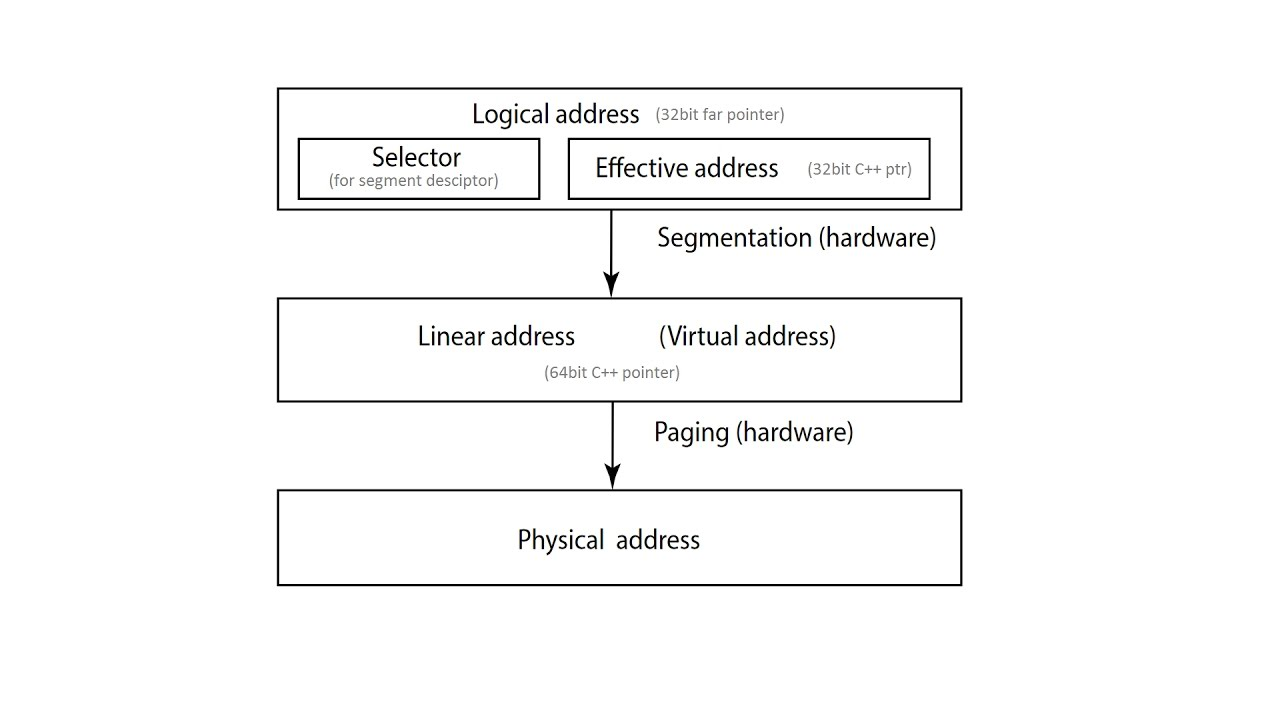
\includegraphics[width=0.8\linewidth]{figure/virtual_linear_physical_address}
\end{figure}

\subsubsection{Exercise \Rmnum{5}}
\begin{flushleft}
{\Large Question}
\end{flushleft}

GDB can only access QEMU's memory through virtual addresses, but when learning to create virtual addresses, we also need to check the physical address at the same time. Learn QEMU's monitor command, especially the xp command, which allows you to check physical memory.

\begin{flushleft}
{\Large Answer}
\end{flushleft}

Open Terminal, enter qemu-system-i386 -hda obj/kern/kernel.img -monitor stdio -gdb tcp::26000 -D qemu.log , after the correct installation, we can use the monitor command.
\begin{figure}[H]
\centering
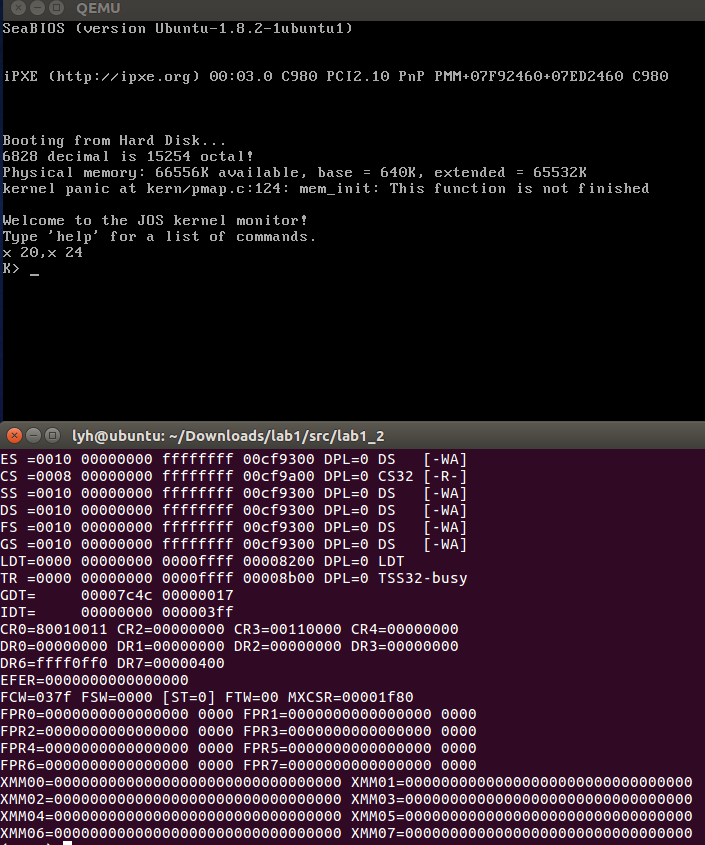
\includegraphics[width=0.8\linewidth]{figure/qemu_commond}
\caption{qemu command}
\end{figure}

\subsubsection{Question \Rmnum{3}}
\begin{flushleft}
{\Large Question}
\end{flushleft}

Assuming the following kernel code is correct, then what type of variable x will be, uintptr\_t or
Physaddr\_t?
\begin{flushleft}
Mystery\_t x;\\
Char* value = return\_a\_pointer();\\
*value = 10; \\
x =(mystery\_t) value;\\
\end{flushleft}
\begin{flushleft}
{\Large Answer}
\end{flushleft}

Since the * operator is used here to resolve the address, the variable x should be of type uintptr\_t.

\subsubsection{Reference counting}
In the previous experiment, we encountered pp\_ref, which records how many different virtual addresses exist on each physical page to reference it. When this value becomes 0, the physical page can be released. In general, the pp\_ref value of any physical page p is equal to the number of times it is mapped by the virtual page under the virtual address UTOP in all page table entries (the address range above UTOP is already mapped at startup) Finished, will not be changed afterwards).

\subsubsection{Page Table Management}
Now we can start writing programs that manage page tables: including inserting and deleting linear address-to-physical address mappings, and creating page tables.

\subsubsection{Homework \Rmnum{4}}
\begin{flushleft}
{\Large Question}\\
In the file kern/pmap.c, you must implement code for the following functions.\\
pgdir\_walk()\\
boot\_map\_region()\\
page\_lookup()\\
page\_remove()\\
page\_insert()\\	
check\_page(), called from mem\_init(), tests your page table management routines. You should make sure it reports success before proceeding.\\
\end{flushleft}
\begin{flushleft}
{\Large Theoretical preparation}
\end{flushleft}

In the previous description, we have a basic understanding of the concept of virtual address, linear address, and physical address.

{\large Physical address}

The unit addressing for the memory chip level corresponds to the address bus to which the processor and the CPU are connected.
- This concept should be the best understood of these concepts. However, it is worth mentioning that although the physical address can be directly understood as the memory itself inserted in the machine, the memory is treated as a large array of numbers from 0 bytes up to the maximum amount of bytes, and then this is An array is called a physical address. However, in fact, this is just an abstraction provided by the hardware to the software. The way memory is addressed is not the case. So, to say that it is "corresponding to the address bus" is more appropriate. Just aside from the consideration of the physical memory addressing mode, it is acceptable to directly compare the physical address with the physical memory. Perhaps the wrong understanding is more conducive to metaphysical abstraction.

{\large Virtual memory}

This is a description of the abstraction of the entire memory (not to the top of the machine).

It is relative to physical memory and can be directly understood as "not straight" and "fake" memory. For example, a 0x08000000 memory address. It is not correct for the address element of 0x08000000 -1 in the large array on the physical address.

The reason is this. Because modern operating systems provide a kind of memory management, that is, virtual memory. The process uses the address in virtual memory, which is assisted by the operating system to "convert" it into a real physical address.

This "conversion". It is the key to all issues discussed.
With this kind of abstraction. A program can use a much larger address space than the real physical address.

Even multiple processes can use the same address. Not surprisingly. Since the converted physical address is not the same.
—— Can decompile the connected program and find that the connector has assigned an address to the program. For example, to call a function A, the code is not call A, but call 0x0811111111, that is, function A The address has been fixed. Without such a "conversion", there is no concept of a virtual address, and doing so is simply not feasible.

{\large Logical address}

In order to be compatible, Intel has retained the segmental memory management method of ancient times.

A logical address is an address used in a machine language instruction to specify an operand or an instruction. In the above example, we say that the address assigned to A by the connector 0x08111111 is the logical address. . "A logical address is an offset of a segment identifier plus a relative address within a specified segment. It is expressed as [segment identifier: offset within segment], that is, the 0x08111111 in the above example should indicate For [A's code segment identifier: 0x08111111], this is complete."

{\large Linear address or virtual address (virtual address)}

Similar to the logical address, it is also an unreal address. If the logical address is the corresponding hardware platform segment management pre-conversion address, then the linear address corresponds to the pre-conversion address of the hardware page memory.

We also need to know the knowledge about the page table.

Our physical memory has a total of 4GB, and we assign it to the page, each page is 4KB in size.

The 4GB (2 to the 32th power) linear address space can be divided into 1048576 (2 to the 20th power, that is, 1M, can also be regarded as 1024 * 1024) pages, so you can randomly extract these pages, every 1024 The pages are a group and can be divided into 1024 groups. For each group of 1024 pages of physical addresses, arranged in a certain order can constitute a table (each entry is the physical address of a page), this table is the page table. The size of the page table is 1024*4B=4KB, which is exactly the size of a physical page.

Because it has been divided into 1024 groups, each group has a page table (size 4KB), so these 1024 page tables can be pointed to by a table, this is the page directory. Similar to the page table, the page directory has a total of 1024 entries (called page directory entries), and the content of each page directory entry is the physical address of a page table. The size of the page table is 1024*4B=4KB, which is exactly the size of a physical page.

The conversion of three addresses and the page table mechanism are shown in the figure below.
\begin{figure}[H]
\centering
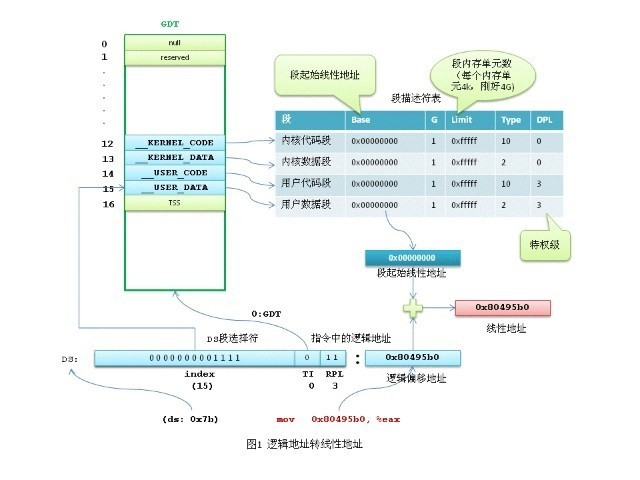
\includegraphics[width=0.8\linewidth]{figure/address_transform_1}
\end{figure}

\begin{figure}[H]
\centering
\includegraphics[width=0.8\linewidth]{figure/address_transform_2}
\end{figure}

\begin{figure}[H]
\centering
\includegraphics[width=0.8\linewidth]{figure/address_transform}
\end{figure}

\begin{flushleft}
{\Large Analysis \& Answer}
\end{flushleft}

By commenting, we can know that the function of this function is given a page directory table pointer pgdir , which should return the page table entry pointer corresponding to the linear address va.We need to complete the transformation as shown in the figure, return the corresponding page table address, that is, the virtual address of the part circled by the red circle:
\begin{figure}[H]
\centering
\includegraphics[width=0.8\linewidth]{figure/pgdir_walk_purpose}
\end{figure}

In addition, we need to understand the meaning of the three parameters.In addition, we need to understand the meaning of the three parameters, pgdir means the page directory item pointer, va means linear address, JOS equals virtual address, create means if page directory entry does not exist or not.

Here we should complete the following steps:

1. Find the page table page where the virtual address is located by the page directory table for the page directory entry address dic\_entry\_ptr in the page directory. (7-8)

2. Determine if the page table page corresponding to this page directory entry is already in memory. (10)

3. If yes, calculate the base address page\_base of this page table page, and then return the address of the page entry corresponding to va \&page\_base[page\_off] (23-25)

4. If not, and create is true, a new page is allocated, and the information of this page is added to the page directory entry dic\_entry\_ptr. (11-18)

5. If create is false, it returns NULL. (19-20)

The modified code is shown in the figure
\begin{figure}[H]
\centering
\includegraphics[width=0.8\linewidth]{figure/pgdir_walk_changed}
\caption{pgdir\_walk}
\end{figure}

Next we complete the boot\_map\_region function. By comment, we can see that the function of this function is to map [va, va+size) of virtual address space to physical [pa, pa+size) in the page table rooted at pgdir.  Size is a multiple of PGSIZE,and va and pa are both page-aligned.Use permission bits perm|PTE\_P for the entries.


The mapping of the virtual address space range [va, va+size) to the physical space [pa, pa+size) is added to the page table pgdir. The main purpose of this function is to set the address range above the virtual address UTOP. The address mapping of this part is static and will not change during the operation of the operating system, so the value of the pp\_ref field in the PageInfo structure of this page. No change will happen.

The steps to be completed by this function are as follows:

Need to complete a loop, using the pgdir\_walk function we just completed, we can use a loop to map all the memory in size bytes.The modified code is shown in the figure:
\begin{figure}[H]
\centering
\includegraphics[width=0.8\linewidth]{figure/boot_map_region_changed}
\caption{boot\_map\_region}
\end{figure}

Next,we continue to view page\_insert(). The function prototype is as follows: page\_insert(pde\_t *pgdir, struct PageInfo *pp, void *va, int perm), which is functionally completed: mapping a page pp in a physical memory to a virtual address va .

The main steps of this function are as follows:

1. First, find the page table entry corresponding to the virtual address va by using the pgdir\_walk function. (4)

2. Modify the value of pp\_ref. (8)

3. Check the page table entry to determine if va has been mapped. If it is mapped, delete the mapping. (9-13)

4. Add the mapping between va and pp to the page table entry. (14-15)

\begin{figure}[H]
\centering
\includegraphics[width=0.8\linewidth]{figure/page_insert_changed}
\caption{page\_insert}
\end{figure}

Next, we complete the page\_lookup function, which functions as return the page mapped at virtual address 'va'.If the pte\_store parameter is not 0, the page table entry address of this physical page is stored in pte\_store.

We only need to call the pgdir\_walk function to get the page table entry corresponding to this va, and then determine whether the page is already in memory, and if so, return the PageInfo structure pointer of this page. And store the contents of this page table entry in pte\_store.The modified code is shown in the figure:
\begin{figure}[H]
\centering
\includegraphics[width=0.8\linewidth]{figure/page_lookup_changed}
\caption{page\_lookup}
\end{figure}

The last one is the page\_remove function. Its prototype is: void page\_remove(pde\_t *pgdir, void *va). The function is to delete the mapping between the virtual address va and the physical page.

The note also hints at a few details to be aware of:

1. The pp\_ref value should be reduced by one.

2. If pp\_ref is reduced to 0, this page should be recycled

3. The page table entry corresponding to this page should be set to 0.

\begin{figure}[H]
\centering
\includegraphics[width=0.8\linewidth]{figure/page_remove_changed}
\caption{page\_remove}
\end{figure}

\subsection{Kernel address space}

JOS divides the 32-bit linear address virtual space into two parts. The user environment (process running environment) usually occupies the part of the low address, called the user address space. The operating system kernel always occupies the part of the high address, called the kernel address space. The dividing line between these two parts is a macro ULIM defined in the memlayout.h file. JOS reserves nearly 256MB of virtual address space for the kernel. This can be understood, why in the experiment 1 to design a high address address space for the operating system. If you don't do this, the address space of the user environment is not enough.

\subsubsection{Homework \Rmnum{5}}
\begin{flushleft}
{\Large Question}
\end{flushleft}
Fill in the missing code in mem\_init() after the call to check\_page().

\begin{flushleft}
{\Large Theoretical preparation}
\end{flushleft}

Since the kernel and user memory are present in the address space of each environment, we need to use the permission bits in the x86 page table to allow the user code to access only the user portion of the address space. Otherwise, bugs in the user code may overwrite the kernel data, causing a crash; or the user code can steal private data from other environments.
The user environment will have no access to any memory above ULIM, and the kernel can read and write this portion of memory. For the address range [UTOP, ULIM), the kernel and the user environment have the same permissions: they can only be read and not written. Under UTOP
The address space is used by the user environment, and the user environment will set permissions to access this part of the memory.
\begin{figure}[H]
\centering
\includegraphics[width=0.8\linewidth]{figure/mem_layout}
\end{figure}

\begin{flushleft}
{\Large Analysis \&Answer}
\end{flushleft}

In this exercise, three virtual addresses are mapped to the physical page.

First, we will complete the UPAGES mapping UPAGES (0xef000000 \~ 0xef400000) up to 4MB, which is the data structure of JOS recording physical page usage.

Currently only one page directory is created, kernel\_pgdir, so the first parameter is obviously kernel\_pgdir. The second parameter is the virtual address, and UPAGES is originally given as a virtual address. The third parameter is the mapped memory block size. The fourth parameter is the physical address mapped to, and the physical address of pages can be taken directly. Permissions PTE\_U indicates that the user has permission to read.Currently only one page directory is created, kernel\_pgdir, so the first parameter is obviously kernel\_pgdir. The second parameter is the virtual address, and UPAGES is originally given as a virtual address. The third parameter is the mapped memory block size. The fourth parameter is the physical address mapped to, and the physical address of pages can be taken directly. Permissions PTE\_U indicates that the user has permission to read.
The modified code is shown in the figure
\begin{figure}[H]
\centering
\includegraphics[width=0.8\linewidth]{figure/mem_init_changed1}
\end{figure}


Then there is the memory stack, the kernel stack ( 0xefff8000 \~ 0xf0000000) 32kB
Bootstrap represents the lowest address of the stack. Since the stack grows to the lower address, it is actually the top of the stack. We will map the address space in [KSTACKTOP-KSTKSIZE, KSTACKTOP)
The modified code is shown in the figure
\begin{figure}[H]
\centering
\includegraphics[width=0.8\linewidth]{figure/mem_init_changed2}
\end{figure}


Finally, the kernel part, we will map the kernel ( 0xf0000000 \~ 0xffffffff ) 256MB
The modified code is shown in the figure
\begin{figure}[H]
\centering
\includegraphics[width=0.8\linewidth]{figure/mem_init_changed3}
\end{figure}

As a result,  the code works successfully.

\begin{figure}[H]
\centering
\includegraphics[width=0.8\linewidth]{figure/make_qemu}
\end{figure}

\begin{figure}[H]
\centering
\includegraphics[width=0.8\linewidth]{figure/make_grade}
\end{figure}

\subsubsection{Question \Rmnum{4}}
\begin{flushleft}
1)\\
What entries (rows) in the page directory have been filled in at this point? What addresses do they map and where do they point? In other words, fill out this table as much as possible:
\begin{figure}[H]
\centering
\includegraphics[width=0.8\linewidth]{figure/question4}
\end{figure}
\end{flushleft}
\begin{flushleft}
{\Large Answer}
\end{flushleft}
\begin{table}[H]
\centering
\begin{tabular}{ |p{150pt}<{\centering}|p{150pt}<{\centering}|p{150pt}<{\centering}| }
\hline				
Entry & Base Virtual Address &Points to(logically) \\ \hline 	
1023 & 0xffc00000 Points to(logically) & Page table for top 4MB of physical memory.This is the last address finding page table that the kernel can use.\\ \hline
1022 & 0xff800000 &Page table for 248MB--(252MB-1)physical memory \\ \hline 	
... & ... &Page table for physical memory \\ \hline
960 & 0xf0000000(KERNBASE) &static data 0--(4MB-1) physical memory \\ \hline
959 & 0xefc00000(VPT) &Page directory self (kernel RW).This is the first page table and it ’ s in the bottom of the physical memory. \\ \hline
958 & 0xef800000(ULIM) &Page table for kernel stack.It is mapped into the physical memory which is the same as bootstack.We only map the memory that the same as KSTACKSIZE.The rest memory that wasn’t mapped is used to avoid the overflow of the kernel stack. \\ \hline
957 & 0xef400000(UVPT) &Same as 959(user kernel R) \\ \hline
956 & 0xef00000(UPAGES) &Page table for structure pages[] \\ \hline
... & ... & NULL \\ \hline
2 & 0x00800000 & NULL \\ \hline
1 & 0x00400000 & NULL \\ \hline
0 & 0x00000000 & The start of the virtual memory .The same as 960(then turn to NULL)\\ \hline
\end{tabular}
\caption{Answer}
\end{table}

\begin{flushleft}
2)We have placed the kernel and user environment in the same address space. Why will user programs not be able to read or write the kernel's memory? What specific mechanisms protect the kernel memory?

{\Large Answer}
\end{flushleft}

User is not allowed to access kernel memory for safety reasons.
If user have the permission, bugs in user code may led to crash.
It is the paging mechanism that protects kernel address in JOS. If the flag bit PTE\_U is 0 in a page, that means user have no permission to read or write the page.

\begin{flushleft}
3)What is the maximum amount of physical memory that this operating system can support? Why?

{\Large Answer}
\end{flushleft}
\begin{figure}[H]
\centering
\includegraphics[width=0.8\linewidth]{figure/question4_3_1}
\caption{PTSIZE}
\end{figure}

\begin{figure}[H]
\centering
\includegraphics[width=0.8\linewidth]{figure/question4_3_2}
\caption{UPAGES}
\end{figure}

\begin{figure}[H]
\centering
\includegraphics[width=0.8\linewidth]{figure/question4_3_3}
\caption{Page}
\end{figure}

2GB.

Pages use up to 4MB space, and each PageInfo use 8Byte. 4M / 8 * 4kB=2GB (4kB per page).


\begin{flushleft}
4)How much space overhead is there for managing memory, if we actually had the maximum amount of physical memory? How is this overhead broken down?

{\Large Answer}

totally 6MB+4KB\\
————————————————————————————————\\
The maximum physical memory is 2G, so there's 0.5M pages in total.\\
8*0.5M = 4MB	(struct PageInfo use 8bytes per page)\\
4*0.5M = 2MB 	(each page table uses 4bytes)\\
4KB		(Page director uses 4kB)\\
————————————————————————————————\\
\end{flushleft}
\clearpage


%============= 参考文献 =====================
%\section*{ \centering 参考文献}
\begin{flushleft}
[1] 位、字、字节的区别 | 汇编伪指令db,dw,dd
[B/OL].http://blog.csdn.net/aurorayqz/article/details/71549166
\par
\vspace{3ex}
[2] MASM32 控制台输入输出
[B/OL].http://blog.csdn.net/xboxmicro/article/details/21658003
\par
\vspace{3ex}
[3] Kip R.Irvine,温玉杰(译),梅广宇(译)等.Intel汇编语言设计(第五版)[M].北京:电子工业出版社,2007
\par
\vspace{3ex}
[4] Jeffrey D.Ullman,Ravi Sethi,Monica S.Lam,Alfred V.Aho.《编译原理》.
机械工业出版社
\end{flushleft}
\addcontentsline{toc}{section}{参考文献}
\clearpage


%\usepackage{cite}
\bibliographystyle{gbt7714-2005}
%\bibliography{bibfile}%%我们的例子应该是\bibliography{cited}
%\newpage
\appendix %添加附录编号

%%附录第一个章节
\section{附录一:factorial.cpp}
\begin{lstlisting}[language={[x86masm]Assembler}]
#include<iostream>
using namespace std;
int main()
{
	//test
	int i,n,f;

	cin>>n;
	i=2;
	f=1;
	while(i<=n)
	{
		f=f*i;
		i=i+1;
	}
	cout<<n<<endl;
	return 0;
}
\end{lstlisting}
\section{附录二:fibonacci.cpp}


%%斐波那契

\begin{lstlisting}[language={c++}]
#include<iostream>
using namespace std;
int main()
{
	int i,n,f;

	cin>>n;
	i=2;
	f=1;
	while(i<=n)
	{
		f=f*i;
		i=i+1;
	}
	cout<<n<<endl;
	return 0;
}

\end{lstlisting}
\clearpage




%\addcontentsline{toc}{section}{附录二:阶乘}



%=============  致谢  ======================





\end{document}
%%%%%%%%%% 结束 %%%%%%%%%%
